\newpage
% \onecolumn
\appendix


\section{Appendix}
\subsection{Comprehensive experimental setup and results}


\begin{table*}[h]
\centering
\resizebox{\textwidth}{!}{
 \begin{tabular}{l *{24}{c}}
    \toprule
 & \multicolumn{3}{c}{Game24} & \multicolumn{3}{c}{HamCycle} & \multicolumn{3}{c}{HamPath} & \multicolumn{3}{c}{Hitori} & \multicolumn{3}{c}{Maze(E)} & \multicolumn{3}{c}{Maze(H)} & \multicolumn{3}{c}{AIME24-25} & \multicolumn{3}{c}{Overall} \\
    \textbf{Checkpoint} & S & U & M & S & U & M & S & U & M & S & U & M & S & U & M & S & U & M & S & U & M & $\mathrm{S}$ & $\mathrm{U}$ & $\mathrm{M}$ \\
\midrule
Deepseek-V3.2-R & 98.0 & 77.5 & 87.8 & 83.5 & 94.0 & 88.8 & 84.0 & 96.0 & 90.0 & 70.0 & 86.0 & 78.0 & 100.0 & 98.9 & 99.5 & 98.0 & 98.0 & 98.0 & 85.0 & 40.3 & 62.7 & 88.4 & 84.4 & 86.5 \\
Gemini-3.0-Pro & 94.0 & 94.0 & 94.0 & 100.0 & 98.0 & 99.0 & 100.0 & 90.0 & 95.0 & 98.0 & 100.0 & 99.0 & 99.0 & 94.6 & 96.8 & 96.0 & 91.0 & 93.5 & 95.0 & 21.2 & 58.1 & 97.4 & 84.1 & 90.8 \\
\midrule
Qwen3-4B-Instruct & 81.0 & 17.0 & 49.0 & 37.5 & 57.0 & 47.3 & 37.0 & 56.5 & 46.8 & 34.5 & 6.5 & 20.5 & 32.7 & 55.6 & 44.1 & 13.3 & 64.5 & 38.9 & 67.9 & 14.8 & 41.4 & 43.4 & 38.8 & 41.1 \\
 + Mix Tag & 82.0 & \sout{92.0} & 87.0 & 31.3 & \sout{100.0} & 66.0 & 38.0 & \sout{100.0} & 69.0 & 48.0 & \sout{90.0} & 69.0 & 85.0 & \sout{91.5} & 88.2 & 33.0 & \sout{84.0} & 58.5 & 58.3 & \sout{61.3} & 59.8 & 53.7 & \sout{88.4} & \sout{71.1} \\
 + TruthRL & 91.0 & 91.0 & 91.0 & 32.3 & 86.0 & 59.2 & 49.0 & 90.0 & 69.5 & 38.0 & 15.0 & 26.5 & 90.0 & 77.1 & 83.6 & 31.0 & 56.5 & 43.8 & 67.5 & 19.1 & 43.3 & 57.0 & 62.1 & 59.6 \\
 + w/o UnsData w/o P & 83.0 & 92.0 & 87.5 & 36.5 & 81.0 & 58.8 & 47.0 & 84.0 & 65.5 & 46.0 & 20.0 & 33.0 & 88.5 & 76.6 & 82.6 & 34.5 & 60.5 & 47.5 & 68.3 & 24.0 & 46.2 & 57.7 & 62.6 & 60.2 \\
 + w/o UnsData w/ P & 90.5 & 12.5 & 51.5 & 39.6 & 67.5 & 53.5 & 49.5 & 64.5 & 57.0 & 56.5 & 4.0 & 30.3 & 94.8 & 83.2 & 89.0 & 56.3 & 72.0 & 64.1 & 69.0 & 7.4 & 38.2 & 65.2 & 44.4 & 54.8 \\
 + w/ UnsData w/o P & 84.0 & 95.0 & 89.5 & 39.6 & 96.0 & 67.8 & 53.0 & 100.0 & 76.5 & 45.0 & 87.0 & 66.0 & 95.5 & 95.2 & 95.4 & 40.0 & 89.5 & 64.8 & 67.1 & 30.8 & 49.0 & 60.6 & 84.8 & 72.7 \\
 + w/ UnsData w/ P & 88.0 & 97.0 & 92.5 & 35.9 & 95.5 & 65.7 & 51.5 & 99.5 & 75.5 & 48.5 & 71.0 & 59.8 & 94.0 & 95.5 & 94.8 & 53.3 & 79.8 & 66.6 & 66.9 & 31.9 & 49.4 & 62.6 & 81.5 & 72.0 \\
 + Fixed-$\tau$ Final & 87.5 & 99.0 & 93.3 & 39.1 & 100.0 & 69.6 & 67.0 & 99.5 & 83.3 & 51.0 & 98.0 & 74.5 & 96.3 & 100.0 & 98.2 & 52.5 & 95.8 & 74.2 & 69.0 & 41.9 & 55.5 & 66.1 & 90.6 & 78.4 \\
 + w/ UnsData w/ P Final & 94.5 & 99.0 & 96.8 & 41.1 & 94.5 & 67.8 & 55.0 & 96.5 & 75.8 & 63.5 & 94.5 & 79.0 & 96.5 & 98.9 & 97.7 & 65.8 & 89.0 & 77.9 & 69.6 & 40.4 & 55.0 & 69.4 & 87.5 & 78.6 \\
\midrule
Qwen3-1.7B-Instruct & 78.0 & 23.0 & 50.5 & 22.9 & 28.0 & 25.5 & 14.0 & 33.0 & 23.5 & 8.0 & 21.0 & 14.5 & 0.0 & 85.6 & 42.8 & 0.0 & 80.0 & 40.0 & 38.3 & 21.2 & 29.8 & 23.0 & 41.7 & 32.4 \\
 + TruthRL & 76.0 & 80.0 & 78.0 & 19.8 & 49.0 & 34.4 & 17.0 & 58.0 & 37.5 & 4.0 & 25.0 & 14.5 & 1.5 & 82.4 & 42.0 & 0.0 & 73.5 & 36.8 & 42.1 & 17.0 & 29.6 & 22.9 & 55.0 & 39.0 \\
 + w/o UnsData w/o P & 77.0 & 88.0 & 82.5 & 25.0 & 60.0 & 42.5 & 15.0 & 83.0 & 49.0 & 5.0 & 53.0 & 29.0 & 0.5 & 93.6 & 47.1 & 0.0 & 79.5 & 39.8 & 32.9 & 24.4 & 28.7 & 22.2 & 68.8 & 45.5 \\
 + w/o UnsData w/ P & 85.0 & 2.0 & 43.5 & 22.4 & 10.5 & 16.5 & 25.5 & 14.0 & 19.8 & 12.0 & 2.5 & 7.3 & 0.0 & 0.0 & 0.0 & 0.0 & 0.0 & 0.0 & 40.8 & 0.5 & 20.7 & 26.5 & 4.2 & 15.4 \\
 + w/ UnsData w/o P & 70.0 & 97.0 & 83.5 & 22.9 & 94.0 & 58.5 & 22.0 & 97.0 & 59.5 & 4.0 & 79.0 & 41.5 & 0.5 & 95.2 & 47.9 & 0.0 & 86.0 & 43.0 & 31.7 & 46.8 & 39.3 & 21.6 & 85.0 & 53.3 \\
 + w/ UnsData w/ P & 82.0 & 96.5 & 89.3 & 18.2 & 85.0 & 51.6 & 20.5 & 89.5 & 55.0 & 8.0 & 62.0 & 35.0 & 0.0 & 90.7 & 45.4 & 0.0 & 74.3 & 37.2 & 40.8 & 21.2 & 31.0 & 24.2 & 74.2 & 49.2 \\
 + w/ UnsData w/ P Final & 84.0 & 100.0 & 92.0 & 20.8 & 88.0 & 54.4 & 27.0 & 85.0 & 56.0 & 11.0 & 59.0 & 35.0 & 0.0 & 95.2 & 47.6 & 0.0 & 79.0 & 39.5 & 35.4 & 28.7 & 32.1 & 25.5 & 76.4 & 50.9 \\
\midrule
Llama3-8B-Distill & 28.0 & 48.0 & 38.0 & 27.1 & 2.0 & 14.6 & 14.0 & 0.0 & 7.0 & 6.0 & 56.0 & 31.0 & 1.0 & 44.7 & 22.9 & 0.0 & 52.0 & 26.0 & 35.0 & 39.4 & 37.2 & 15.9 & 34.6 & 25.2 \\
 + Mix Tag & 2.0 & \sout{96.0} & 49.0 & 18.8 & \sout{98.0} & 58.4 & 22.0 & \sout{100.0} & 61.0 & 2.0 & \sout{100.0} & 51.0 & 23.0 & \sout{78.7} & 50.8 & 1.0 & \sout{85.0} & 43.0 & 35.8 & \sout{80.8} & 58.3 & 14.9 & \sout{91.2} & \sout{53.1} \\
 + w/o UnsData w/o P  & 58.0 & 2.0 & 30.0 & 41.7 & 0.0 & 20.8 & 50.0 & 0.0 & 25.0 & 6.0 & 2.0 & 4.0 & 67.0 & 7.4 & 37.2 & 8.0 & 8.0 & 8.0 & 46.7 & 9.6 & 28.1 & 39.6 & 4.1 & 21.9 \\
 + w/ UnsData w/ P & 66.0 & 4.0 & 35.0 & 39.6 & 98.0 & 68.8 & 48.0 & 90.0 & 69.0 & 10.0 & 78.0 & 44.0 & 60.0 & 3.2 & 31.6 & 7.0 & 20.0 & 13.5 & 50.0 & 30.9 & 40.5 & 40.1 & 46.3 & 43.2 \\
 + w/ UnsData w/ P Final & 80.0 & 22.0 & 51.0 & 52.1 & 100.0 & 76.1 & 74.0 & 92.0 & 83.0 & 30.0 & 76.0 & 53.0 & 67.0 & 42.6 & 54.8 & 13.0 & 35.0 & 24.0 & 43.3 & 44.7 & 44.0 & 51.3 & 58.9 & 55.1 \\
% \midrule
\bottomrule
\end{tabular}}
\caption{Detailed performance breakdown (S/U/M) across all seven datasets. This table lists the full experimental results for all baselines and Qwen3 variants (including ablation checkpoints and final converged models). S: Solvable Accuracy; U: Unsolvable Detection Rate; M: Mean Score.}
\label{tab:results_per_domain_app}
\end{table*}


% [Table A2 Code]
\begin{table*}[h]
\centering
\resizebox{\textwidth}{!}{
\begin{tabular}{l *{24}{c}}
\toprule
 & \multicolumn{3}{c}{Game24} & \multicolumn{3}{c}{HamCycle} & \multicolumn{3}{c}{HamPath} & \multicolumn{3}{c}{Hitori} & \multicolumn{3}{c}{Maze(E)} & \multicolumn{3}{c}{Maze(H)} & \multicolumn{3}{c}{AIME24-25} & \multicolumn{3}{c}{Overall} \\
        \textbf{Checkpoint} & Corr & Rej & C+R & Corr & Rej & C+R & Corr & Rej & C+R & Corr & Rej & C+R & Corr & Rej & C+R & Corr & Rej & C+R & Corr & Rej & C+R & Corr & Rej &C+R \\
\midrule
Deepseek-V3.2-R & 87.8 & 0.00 & 87.8 & 88.8 & 8.30 & 97.1 & 90.0 & 6.00 & 96.0 & 78.0 & 9.00 & 87.0 & 99.5 & 0.00 & 99.5 & 98.0 & 0.00 & 98.0 & 62.7 & 0.80 & 63.5 & 86.5 & 3.44 & 90.0 \\
Gemini-3.0-Pro & 94.0 & 1.00 & 95.0 & 99.0 & 0.00 & 99.0 & 95.0 & 0.00 & 95.0 & 99.0 & 0.00 & 99.0 & 96.8 & 0.00 & 96.8 & 93.5 & 0.00 & 93.5 & 58.1 & 0.00 & 58.1 & 90.8 & 0.14 & 90.9 \\
\midrule
Qwen3-4B-Instruct & 49.0 & 0.00 & 49.0 & 47.3 & 24.74 & 72.0 & 46.8 & 12.00 & 58.8 & 20.5 & 4.00 & 24.5 & 44.1 & 0.00 & 44.1 & 38.9 & 0.25 & 39.2 & 41.4 & 0.00 & 41.4 & 41.1 & 5.86 & 47.0 \\
 + TruthRL & 91.0 & 0.50 & 91.5 & 59.2 & 34.15 & 93.4 & 69.5 & 16.00 & 85.5 & 26.5 & 18.50 & 45.0 & 83.6 & 2.50 & 86.1 & 43.8 & 11.00 & 54.8 & 43.3 & 0.00 & 43.3 & 59.6 & 11.81 & 71.4 \\
 + w/o UnsData w/o P & 87.5 & 0.00 & 87.5 & 58.8 & 28.85 & 87.7 & 65.5 & 15.50 & 81.0 & 33.0 & 11.00 & 44.0 & 82.6 & 0.00 & 82.6 & 47.5 & 0.00 & 47.5 & 46.2 & 0.00 & 46.2 & 60.2 & 7.91 & 68.1 \\
 + w/o UnsData w/ P & 51.5 & 0.00 & 51.5 & 53.5 & 21.09 & 74.6 & 57.0 & 7.00 & 64.0 & 30.3 & 2.25 & 32.6 & 89.0 & 0.00 & 89.0 & 64.1 & 0.13 & 64.2 & 38.2 & 0.00 & 38.2 & 54.8 & 4.35 & 59.2 \\
 + w/ UnsData w/o P & 89.5 & 1.50 & 91.0 & 67.8 & 19.00 & 86.8 & 76.5 & 10.00 & 86.5 & 66.0 & 13.00 & 79.0 & 95.4 & 1.00 & 96.4 & 64.8 & 4.00 & 68.8 & 49.0 & 0.42 & 49.4 & 72.7 & 7.00 & 79.7 \\
 + w/ UnsData w/ P & 92.5 & 1.00 & 93.5 & 65.7 & 19.75 & 85.5 & 75.5 & 15.50 & 91.0 & 59.8 & 7.50 & 67.3 & 94.8 & 0.00 & 94.8 & 66.6 & 1.00 & 67.6 & 49.4 & 0.00 & 49.4 & 72.0 & 6.39 & 78.4 \\
 + Fixed-$\tau$ Final & 93.3 & 0.00 & 93.3 & 69.6 & 18.49 & 88.1 & 83.3 & 12.00 & 95.3 & 74.5 & 0.00 & 74.5 & 98.2 & 0.00 & 98.2 & 74.2 & 0.00 & 74.2 & 55.5 & 0.00 & 55.5 & 78.4 & 4.36 & 82.8 \\
 + w/ UnsData w/ P Final & 96.8 & 0.00 & 96.8 & 67.8 & 26.82 & 94.6 & 75.8 & 19.00 & 94.8 & 79.0 & 2.25 & 81.3 & 97.7 & 0.00 & 97.7 & 77.1 & 0.00 & 77.1 & 55.0 & 0.00 & 55.0 & 78.6 & 6.87 & 85.5 \\
\midrule
Qwen3-1.7B-Instruct & 50.5 & 0.00 & 50.5 & 25.5 & 8.85 & 34.3 & 23.5 & 12.00 & 35.5 & 14.5 & 0.50 & 15.0 & 42.8 & 0.00 & 42.8 & 40.0 & 0.00 & 40.0 & 29.8 & 0.00 & 29.8 & 32.4 & 3.05 & 35.5 \\
 + TruthRL & 78.0 & 2.00 & 80.0 & 34.4 & 29.58 & 64.0 & 37.5 & 39.50 & 77.0 & 14.5 & 16.50 & 31.0 & 42.0 & 12.78 & 54.8 & 36.8 & 24.00 & 60.8 & 29.6 & 5.68 & 35.3 & 39.0 & 18.58 & 57.6 \\\
 + w/o UnsData w/o P & 82.5 & 0.50 & 83.0 & 42.5 & 29.17 & 71.7 & 49.0 & 30.00 & 79.0 & 29.0 & 6.50 & 35.5 & 47.1 & 0.25 & 47.3 & 39.8 & 3.50 & 43.3 & 28.7 & 4.17 & 32.9 & 45.5 & 10.58 & 56.1 \\
 + w/o UnsData w/ P & 43.5 & 0.25 & 43.8 & 16.5 & 19.01 & 35.5 & 19.8 & 8.00 & 27.8 & 7.3 & 5.25 & 12.5 & 0.0 & 0.00 & 0.0 & 0.0 & 0.00 & 0.0 & 20.7 & 0.00 & 20.7 & 15.4 & 4.64 & 20.0 \\
 + w/ UnsData w/o P & 83.5 & 1.00 & 84.5 & 58.5 & 22.88 & 81.4 & 59.5 & 19.50 & 79.0 & 41.5 & 2.50 & 44.0 & 47.9 & 1.50 & 49.4 & 43.0 & 0.75 & 43.8 & 39.3 & 2.52 & 41.8 & 53.3 & 7.24 & 60.5 \\
 + w/ UnsData w/ P & 89.3 & 0.00 & 89.3 & 51.6 & 27.77 & 79.4 & 55.0 & 19.50 & 74.5 & 35.0 & 2.50 & 37.5 & 45.4 & 0.00 & 45.4 & 37.2 & 4.50 & 41.7 & 31.0 & 1.46 & 32.5 & 49.2 & 7.96 & 57.2 \\
 + w/ UnsData w/ P Final & 92.0 & 0.50 & 92.5 & 54.4 & 32.19 & 86.6 & 56.0 & 21.50 & 77.5 & 35.0 & 2.00 & 37.0 & 47.6 & 0.55 & 48.2 & 39.5 & 6.75 & 46.3 & 32.1 & 3.17 & 35.3 & 50.9 & 9.52 & 60.4 \\
\midrule
Llama3-8B-Distill & 38.0 & 22.00 & 60.0 & 14.6 & 43.75 & 58.4 & 7.0 & 34.00 & 41.0 & 31.0 & 56.00 & 87.0 & 22.9 & 34.19 & 57.1 & 26.0 & 44.50 & 70.5 & 37.2 & 6.78 & 44.0 & 25.2 & 34.46 & 59.7 \\
 + w/o UnsData w/o P  & 30.0 & 0.00 & 30.0 & 20.8 & 5.21 & 26.0 & 25.0 & 4.00 & 29.0 & 4.0 & 6.00 & 10.0 & 37.2 & 1.00 & 38.2 & 8.0 & 4.00 & 12.0 & 28.1 & 0.83 & 28.9 & 21.9 & 3.01 & 24.9 \\
 + w/ UnsData w/ P & 35.0 & 0.00 & 35.0 & 68.8 & 16.67 & 85.5 & 69.0 & 3.00 & 72.0 & 44.0 & 19.00 & 63.0 & 31.6 & 3.00 & 34.6 & 13.5 & 8.50 & 22.0 & 40.5 & 0.83 & 41.3 & 43.2 & 7.29 & 50.5 \\
 + w/ UnsData w/ P Final & 51.0 & 2.00 & 53.0 & 76.1 & 10.42 & 86.5 & 83.0 & 4.00 & 87.0 & 53.0 & 19.00 & 72.0 & 54.8 & 4.05 & 58.9 & 24.0 & 17.00 & 41.0 & 44.0 & 3.34 & 47.3 & 55.1 & 8.54 & 63.7 \\
% \midrule
\bottomrule
\end{tabular}}
\caption{Alternative metric analysis showing Correctness (\textbf{Corr}), Rejection Rate (\textbf{Rej}), and their sum (\textbf{C+R}). This breakdown distinguishes between general accuracy and refusal tendency, providing a diagnostic view for over-refusal and capability collapse.}
\label{tab:agg_summary_horizontal_app_v2}
\end{table*}
\label{sec:appendix_comprehensive}

In this appendix, we provide the full, domain-level experimental results to supplement the aggregated metrics reported in the main text. Table~\ref{tab:results_per_domain_app} reports the performance breakdown across all seven datasets, including Game24, HamCycle, HamPath, Hitori, Maze-Easy, Maze-Hard, and AIME 24-25. We report three primary metrics to evaluate performance. First, Solvable Accuracy (S) measures the percentage of solvable problems correctly answered. Second, Unsolvable Detection Rate (U) indicates the percentage of unsolvable problems correctly identified as unsolvable. Finally, Mean (M) represents the arithmetic mean of S and U, reflecting the overall reliability of the model across different domains.

Complementing the standard metrics, Table~\ref{tab:agg_summary_horizontal_app_v2} provides a diagnostic view focusing on the model's refusal behavior. Correctness (Corr) measures the accuracy of the model's responses on attempted questions, independent of the refusal decision. Rejection Rate (Rej) tracks the proportion of total queries, including both solvable and unsolvable instances, that the model refused to answer. The sum of these two metrics (C+R) serves as a diagnostic tool to analyze trade-offs between reasoning capability and refusal tendency, helping to identify issues such as over-refusal or capability collapse.

Both tables include results for a wide range of configurations. We compare against strong proprietary models like Deepseek-V3.2-R and Gemini-3.0-Pro, as well as the base Qwen3-Instruct models, which serve as reference points. To isolate the effects of our proposed components, we evaluate ablation variants trained for 120 steps. These include models trained exclusively on solvable data without exposure to ground-truth unsolvable examples (denoted as w/o UnsData) and models trained without the False Unsolvability Penalty (denoted as w/o P), representing standard RLHF without the penalty term for incorrect refusals. Finally, we present results for the fully converged models trained for 320 steps, including a variant using a static confidence threshold (Fixed-tau Final) and our fully converged model trained with the complete UnsolvableRL method (w/ UnsData w/ P Final).

We also extended our evaluation to the Llama3-8B architecture to verify the generalizability of our method. As shown in the tables, training exclusively on solvable data (\textit{w/o UnsData w/o P}) yields a dramatic improvement in solvable accuracy compared to the baseline ($S: 15.9\% \to 39.6\%$). However, this comes at a catastrophic cost: the model's ability to detect unsolvable problems collapses ($U: 34.6\% \to 4.1\%$), leading to a net decline in the overall Mean score ($M: 25.2\% \to 21.9\%$). 

In contrast, our proposed method (\textit{w/ UnsData w/ P}) successfully resolves this conflict. At step 120, it maintains superior solvable accuracy ($S=40.1\%$) while simultaneously robustifying unsolvable detection ($U=46.3\%$), nearly doubling the overall Mean score to 43.2\%. \textbf{Furthermore, extending the training to approximately 400 steps (\textit{Final}) demonstrates robust scalability: the model achieves further gains with Solvable Accuracy reaching 51.3\% and Unsolvable Detection rising to 58.9\%, resulting in a comprehensive Mean score of 55.1\%.} This confirms that UnsolvableRL effectively prevents capability collapse and enhances reasoning rigor across different model families.

\subsection{Analysis of the Conflated Refusal Baseline (+Mix Tag)} \label{sec:mix_tag_analysis}

To further underscore the necessity of decoupling objective detection from subjective calibration, we evaluate a baseline variant referred to as \textit{+Mix Tag}. This model is trained using the exact same dataset and hyperparameter configurations as our full \textit{UnsolvableRL} framework. The critical distinction lies in the prompting strategy: the model is instructed to output a unified \texttt{unsolvable} tag for both objective contradiction detection and subjective difficulty-based refusal, rather than using distinct markers like \texttt{<beyond\_capacity>}.

Under this conflated setting, the reward components defined in Section~\ref{reward_design} are applied based on the ground truth of the instance, even though the model uses a single undifferentiated output:

\begin{itemize}
    \item \textbf{Solvable Instances:} If the model emits the \texttt{unsolvable} tag, it inherently fails to solve the problem, resulting in $R_{\text{acc}} = 0$. However, to prevent the calibration mechanism from collapsing, the system treats this output as a subjective refusal and assigns the dynamic difficulty calibration reward $R_{\text{cal}}$ according to Eq.~\ref{eg_dydc}.
    \item \textbf{Unsolvable Instances:} If the model emits the same \texttt{unsolvable} tag, it is rewarded with the detection signal $R_{\text{detect}} = +1$ (as detailed in Section~\ref{reward_design}), as the unified tag happens to match the objective ground truth of the problem statement.
\end{itemize}

As shown in the \textit{+Mix Tag} row of Table~\ref{tab:results_per_domain_app}, this setup creates a ``reward shortcut'' where the model is incentivized to emit the unified tag to hedge against two different reward sources. Notably, \textbf{after an identical duration of 120 training steps}, this confusion severely suppresses the model's incentive to attempt reasoning across different architectures. Consequently, within this \textbf{fixed budget of 120 steps}, the accuracy on solvable problems ($S$) reaches only 53.7\% for Qwen3-4B and a mere 14.9\% for Llama3-8B. Compared to the 62.6\% (Qwen) and 40.1\% (Llama) achieved by our decoupled method at the same training stage, the conflated approach results in a catastrophic reasoning deficit, particularly evident in the Llama model.

\paragraph{Explanation of Strikethroughs in Table~\ref{tab:results_per_domain_app}.} 
We have applied strikethroughs to the Unsolvable Detection Rate ($U$) and the resulting Mean Score ($M$) for the \textit{+Mix Tag} row. These metrics are confounded and analytically meaningless in this context because the \texttt{unsolvable} tag no longer functions as a specific indicator of logical contradiction. In this undifferentiated regime, the high $U$ scores (e.g., 91.2\% for Llama3-8B and 88.4\% for Qwen3-4B) do not represent superior logical rigor, but rather a mixture of valid detection and ``lazy'' refusal to avoid potential penalties. Furthermore, this conflation diminishes real-world utility: users cannot discern whether the model refused because the query was fundamentally flawed or because it simply lacked the capacity to solve it.

\subsection{Calibration Analysis}
\label{sec:calibration_analysis}
\begin{figure*}[t]
    \centering
    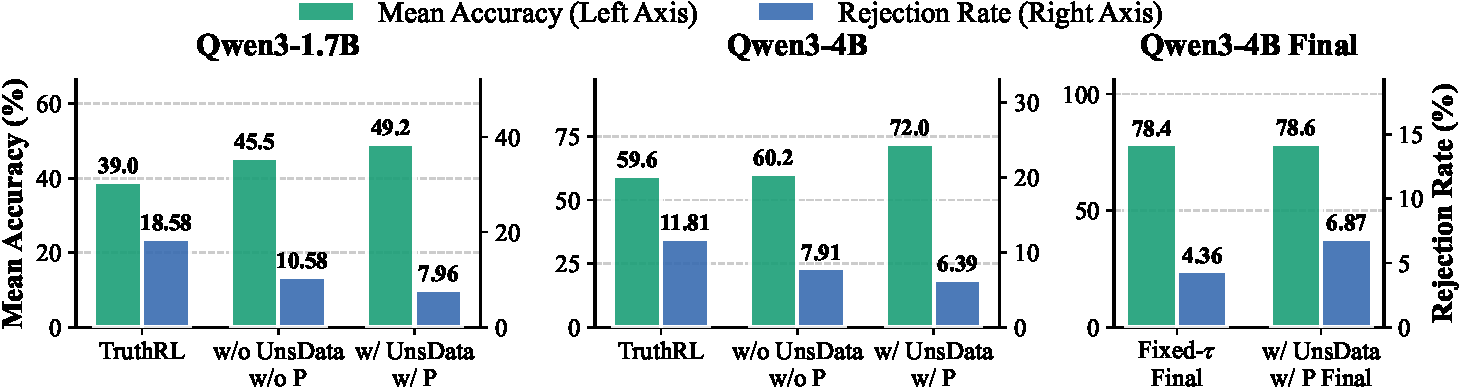
\includegraphics[width=1.0\linewidth]{figures/0105rej_rate_comparison.pdf}
    \caption{
        Performance Comparison and Calibration Analysis. 
        (Left/Middle) Comparison with TruthRL. While TruthRL achieves higher rejection rates (Blue bars), it suffers from over-refusal, significantly degrading Accuracy (Green bars).
        (Right) Comparison of threshold strategies. The adaptive mechanism (\textit{w/ P Final}) maintains a healthier rejection rate (6.87\%) compared to the Fixed-$\tau$ baseline (4.36\%) while preserving high accuracy.
    }
    \label{fig:performance_comparison}
\end{figure*}

\subsection{Details of Diagnostic Dataset Construction}
\label{sec:appendix_data_detail}

To support the fine-grained diagnostic experiments described in Section~\ref{sec:diagnostic_reasoning}, we curated a multi-domain dataset designed to evaluate a model's capability to categorize reasoning failures into two diagnostic families: \textbf{Missing Information (MI)}, which denotes missing support needed for a determinate answer under the requested response format; and \textbf{Constraint Conflict (CC)}, which introduces mutually incompatible conditions within a problem statement.

The diagnostic framework utilizes a rigorous split between training and evaluation to assess both cross-domain and temporal generalization. The training set comprises 259 instances, consisting of 140 multiple-choice problems from the MMLU-Pro validation seeds (70 solvable and 70 unsolvable) and 119 mathematical reasoning tasks derived from AIME 1983 (50 solvable and 69 unsolvable MI/CC instances). To establish a robust evaluation of out-of-distribution (OOD) performance, we constructed a test set of 320 instances using seeds entirely distinct from the training data. This includes 149 instances from the 2024--2025 AIME partitions (60 solvable and 89 unsolvable MI/CC instances) to test temporal generalization and 171 instances from GPQA to evaluate cross-domain transferability. The comprehensive breakdown of these datasets, including solvable and unsolvable distributions, is summarized in Table~\ref{tab:diagnostic_stats_detail}.

\begin{table}[h]
\centering
\small
\resizebox{\columnwidth}{!}{ % 强制缩放到栏宽
\begin{tabular}{llccc}
\toprule
\textbf{Split} & \textbf{Source} & \textbf{Solv.} & \textbf{Unsolv.} & \textbf{Total} \\
\midrule
\multirow{2}{*}{Train} & MMLU-Pro & 70 & 70 & 140 \\
 & AIME (1983) & 50 & 69 & 119 \\
\cmidrule(lr){2-5}
 & \textit{Train Total} & \textit{120} & \textit{139} & \textit{259} \\
\midrule
\multirow{2}{*}{OOD Test} & AIME (24--25) & 60 & 89 & 149 \\
 & GPQA & 100 & 71 & 171 \\
\cmidrule(lr){2-5}
 & \textit{Test Total} & \textit{160} & \textit{160} & \textit{320} \\
\bottomrule
\end{tabular}
}
\caption{Detailed dataset statistics for fine-grained diagnostic reasoning.}
\label{tab:diagnostic_stats_detail}
\end{table}


\subsection{Benchmarking SOTA Models on Diagnostic Reasoning}
To establish a rigorous baseline and demonstrate the inherent difficulty of fine-grained unsolvability diagnosis, we benchmarked state-of-the-art (SOTA) large language models alongside our aligned open-source models on two Out-of-Distribution (OOD) test sets. The first is the 89 unsolvable MI/CC instances from our AIME (2024--2025) set (47 MI and 42 CC). The second is the 71 unsolvable instances from our GPQA dataset (GPQA-U).

We evaluated DeepSeek, Gemini, and GPT-5.2, alongside the baseline and diagnostic-tuned versions of Qwen3-4B and Llama3-8B. The metric of interest is \textit{Diagnostic Accuracy} (the ability to correctly identify the specific root cause of unsolvability or explicitly reject the flawed query). The comprehensive results are presented in Table~\ref{tab:sota_diagnostic_full}.

\begin{table*}[t] % 使用 table* 跨双栏显示大表
\centering
\small
\resizebox{\textwidth}{!}{ 
\begin{tabular}{l cc cc ccc}
\toprule
\multirow{3}{*}{\textbf{Dataset Subset}} & \multicolumn{4}{c}{\textbf{Aligned Open-Source Models}} & \multicolumn{3}{c}{\textbf{Proprietary SOTA Models}} \\
\cmidrule(lr){2-5} \cmidrule(lr){6-8}
 & \multicolumn{2}{c}{\textbf{Qwen3-4B}} & \multicolumn{2}{c}{\textbf{Llama3-8B}} & \multirow{2}{*}{\textbf{DeepSeek}} & \multirow{2}{*}{\textbf{Gemini}} & \multirow{2}{*}{\textbf{GPT-5.2}} \\
 \cmidrule(lr){2-3} \cmidrule(lr){4-5}
 & Instruct & + Diag. & Distill & + Diag. & & & \\
\midrule
\multicolumn{8}{l}{\textit{AIME (2024--2025) Defect Families}} \\
Missing Information (MI) & 23.4 & 41.4 & 38.3 & 38.8 & 51.1 & 46.8 & \textbf{55.3} \\
Constraint Conflict (CC) & 45.2 & 69.6 & 45.2 & \textbf{75.6} & 71.4 & 47.6 & \textbf{76.2} \\
\midrule
\multicolumn{8}{l}{\textit{General Science Defects}} \\
GPQA-U  & 21.7 & 33.8 & 21.5 & \textbf{36.6} & 29.6 & 23.9 & 28.2 \\
\bottomrule
\end{tabular}}
\caption{Comprehensive diagnostic performance (\%) across all evaluated models on OOD unsolvable instances. The table juxtaposes our aligned open-source models (4B/8B) against massive proprietary SOTA models. Note how diagnostic tuning (\textit{+Diag.}) enables smaller models to bridge the gap and occasionally surpass SOTA baselines (e.g., Llama3-8B on CC and GPQA-U).}
\label{tab:sota_diagnostic_full}
\end{table*}

The empirical results reveal several critical insights into current LLM capabilities and the efficacy of our method:

First, \textbf{diagnostic tuning enables small models to rival giants}. Remarkably, explicit diagnostic alignment enables small open-source models to match or exceed massive proprietary systems on targeted tasks. For instance, Llama3-8B (+Diag.) achieves a 75.6\% detection rate on AIME Constraint Conflicts (CC), surpassing DeepSeek (71.4\%) and matching GPT-5.2 (76.2\%). Furthermore, on the graduate-level GPQA-U set, our tuned Llama3-8B (36.6\%) outperforms all evaluated SOTA models.

Second, there is a \textbf{stark variance across defect families in SOTA models}. While models like GPT-5.2 and DeepSeek perform reasonably well on explicit Constraint Conflicts ($>70\%$ accuracy), their performance drops to around 50\% for Missing Information. This suggests that current proprietary models rely heavily on surface-level logical conflicts (e.g., mutually exclusive rules) but struggle to independently verify whether a problem provides sufficient parameters for a determinate answer. This capability gap underscores the necessity of explicit diagnostic alignment frameworks like UnsolvableRL.

\subsection{Out-of-Distribution (OOD) Generalization}
\label{sec:appendix_ood}

To evaluate the generalization capabilities of UnsolRL, we utilized two Out-of-Distribution (OOD) benchmarks: \textbf{8-Puzzle} ($N_{sol}=87, N_{unsol}=100$) and \textbf{Zebra Logic} ($N_{sol}=100, N_{unsol}=100$). These tasks differ significantly from the training distribution, serving as a rigorous test for reasoning robustness. Table~\ref{tab:ood_single_column_trimmed} details the performance mean@4 across Solvable (\textbf{S}), Unsolvable (\textbf{U}), and Mean (\textbf{M}) metrics. 

\paragraph{SOTA Model Performance.}
We first established a baseline using top-tier proprietary models. \textbf{Deepseek-V3.2-R} achieves the highest overall performance (\textbf{M}=76.2\%), demonstrating exceptional dominance in logic tasks with a mean score of 92.7\% on Zebra Logic. In contrast, \textbf{Gemini-3.0-Pro} excels in procedural planning, securing the top spot on the 8-Puzzle benchmark (\textbf{M}=70.3\%). \textbf{GPT-5.2-Low} shows balanced capabilities, particularly in detecting unsolvable instances across both domains (Overall \textbf{U}=94.3\%). These results highlight that while leading models perform well, handling both logical constraints and path-finding robustly remains a non-trivial challenge.

\paragraph{Qwen3-4B Results.} 
The baseline Qwen3-4B model struggles significantly with OOD detection, failing completely to identify unsolvable 8-Puzzle instances (0.0\%). \textbf{UnsolRL-Final} substantially enhances robustness: it raises the \textbf{U} score to 15.8\% on the 8-Puzzle and achieves a remarkable improvement on Zebra Logic, boosting \textbf{U} from 69.0\% to 87.0\%. Consequently, the Overall Mean (\textbf{M}) increases by over 50\% relative to the baseline (from 23.2\% to 34.9\%), demonstrating that our method successfully transfers verification capabilities to unseen tasks.

\paragraph{Llama3-8B Results.}
Similarly, \textbf{Llama3-8B} exhibits substantial gains following UnsolRL alignment. The baseline model shows nearly no competence on the 8-Puzzle ($M=1.0\%$), whereas the aligned version achieves a ten-fold improvement in mean performance ($10.1\%$). On Zebra Logic, it maintains a robust unsolvable detection rate (78.0\%) while doubling its solving accuracy ($1.5\% \to 4.0\%$). Overall, Llama3-8B's mean OOD score rises from 20.4\% to 25.6\%, confirming the cross-architecture efficacy of our reinforcement learning framework.

\paragraph{Qwen3-1.7B Results.} 
Despite its limited capacity, the 1.7B model exhibits a similar positive trend in anomaly detection. On Zebra Logic, UnsolRL improves the unsolvable detection rate (\textbf{U}) from 36.0\% to 47.3\%. Although the complex 8-Puzzle remains highly challenging for this smaller architecture (Overall \textbf{M} for 8-Puzzle improves marginally to 1.1\%), the improvement in the Overall Mean across tasks (from 11.5\% to 13.8\%) confirms that UnsolRL effectively mitigates hallucinations on unsolvable queries, even when reasoning resources are constrained.

\begin{table*}[h]
\centering
\small 
\begin{tabular}{l *{3}{c} *{3}{c} *{3}{c}}
    \toprule
    & \multicolumn{3}{c}{\textbf{8-Puzzle}} & \multicolumn{3}{c}{\textbf{Zebra Logic}} & \multicolumn{3}{c}{\textbf{Overall}} \\
    \cmidrule(lr){2-4} \cmidrule(lr){5-7} \cmidrule(lr){8-10}
    \textbf{Model} & S & U & M & S & U & M & S & U & M \\
    \midrule
    Deepseek-V3.2-R  & 40.2 & 79.0 & 59.6 & \textbf{94.5} & 91.0 & \textbf{92.7} & \textbf{67.3} & 85.0 & \textbf{76.2}\\
    Gemini-3.0-Pro  & \textbf{43.6}& \textbf{97.0} & \textbf{70.3} & 65.0 & 74.0 & 69.5 & 54.3 & 85.5 & 69.9 \\
    GPT-5.2-Low  & 40.8 & 96.0 & 68.4 & 70.0 & \textbf{92.5} & 81.3 & 55.4 & \textbf{94.3} & 74.8 \\

    \midrule
    % --- 4B Group ---
    Qwen3-4B-Instruct & 21.6 & 0.0 & 10.8 & 2.0 & 69.0 & 35.5 & 11.8 & 34.5 & 23.2 \\
    + UnsolRL-Final   & \textbf{26.4} & \textbf{15.8} & \textbf{20.1} & \textbf{8.8} & \textbf{87.0} & \textbf{47.9} & \textbf{17.4} & \textbf{52.4} & \textbf{34.9} \\
    \midrule
    % --- 1.7B Group ---
    Qwen3-1.7B-Instruct & 0.8 & 0.0 & 0.4 & \textbf{9.0} & 36.0 & 22.5 & \textbf{4.9} & 18.0 & 11.5 \\
    + UnsolRL-Final     & \textbf{1.2} & \textbf{1.0} & \textbf{1.1} & 5.3 & \textbf{47.3} & \textbf{26.3} & 3.3 & \textbf{24.2} & \textbf{13.8} \\
    \midrule
    % --- Llama Group ---
    Llama3-8B-Distill & 1.1 & 1.0 & 1.0 & 1.5 & 78.0 & 39.8 & 1.3 & 39.5 & 20.4 \\
    + UnsolRL-Final  & \textbf{10.3} & \textbf{10.0} & \textbf{10.1} & \textbf{4.0} & 78.0 & \textbf{41.0} & \textbf{7.2} & \textbf{44.0} & \textbf{25.6} \\
    \bottomrule
\end{tabular}
\caption{OOD performance. \textbf{S}: Solvable Accuracy, \textbf{U}: Unsolvable Detection Rate, \textbf{M}: Mean Accuracy (\%).}
\label{tab:ood_single_column_trimmed}
\end{table*}

\subsection{Case Study}

To qualitatively demonstrate the effectiveness of our alignment strategy, we present three representative cases generated by \textbf{DeepSeek-V3.2-R}. These examples illustrate the model's ability to navigate complex reasoning paths: detecting latent contradictions in mathematics (Case 1), identifying topological impossibility in logic puzzles (Case 2), and maintaining flexible reasoning for solvable problems (Case 3).

% --- Case 1: AIME ---
\subsubsection*{Case 1: Latent Unsolvability (Number Theory)}

\paragraph{Problem Input.} 
Let $N$ be the greatest four-digit positive integer with the property that whenever one of its digits is changed to $1$, the resulting number is divisible by $7$. Suppose that $N \equiv Q+R \pmod{7}$, where $Q$ and $R$ are the quotient and remainder when $N$ is divided by $1000$. Find $Q+R$.

\paragraph{Original Model Response.}
\begin{quote}
\small
\textit{``The digit-change property requires that for any digit of $N$, replacing that digit with 1 results in a number divisible by 7. Under the strict interpretation... the only solutions are $N = 5624$ and $N = 5694$, with the latter being the greatest.
However, for $N = 5694$, computing $Q = 5$ and $R = 694$ gives $Q + R = 699$. Checking the congruence $N \equiv Q + R \pmod{7}$ yields $5694 \equiv 3 \pmod{7}$ and $699 \equiv 6 \pmod{7}$, which are not equal. ... Thus, the greatest $N$ satisfying the digit-change property does not satisfy the additional condition. Therefore, no four-digit $N$ meets all the requirements.''}
\[ \boxed{\text{unsolvable}} \]
\end{quote}

\paragraph{Reasoning Analysis.} 
This case exemplifies \textbf{"Verify-then-Conclude"}. The contradiction is not explicit in the problem statement but lies deep within the solution space.
\begin{itemize}
    \item \textbf{Deep Execution:} The model does not reject the problem early. It successfully solves the core number theory challenge, identifying the unique candidate $N=5694$.
    \item \textbf{Constraint Verification:} Instead of hallucinating a match, it rigorously computes the modular arithmetic ($3 \neq 6$) and identifies the conflict between the derived candidate and the final constraint.
\end{itemize}

% --- Case 2: Hitori ---
\subsubsection*{Case 2: Topological Impossibility (Hitori)}

\paragraph{Problem Input.} 
Solve the following $4 \times 4$ Hitori puzzle. Rules: No duplicates in rows/cols; Black cells cannot touch; White cells must be connected.
\begin{center}
\small
\setlength{\tabcolsep}{4pt}
\begin{tabular}{|c|c|c|c|}
\hline
4 & 2 & \textbf{3} & \textbf{3} \\ \hline
2 & 1 & 4 & \textbf{2} \\ \hline
4 & 3 & 3 & 2 \\ \hline
4 & 1 & 2 & \textbf{2} \\ \hline
\end{tabular}
\end{center}

\paragraph{Original Model Response.}
\begin{quote}
\small
\textit{``The puzzle is unsolvable due to the isolation of cell (0,3) in all valid configurations... Specifically, the triplet of 2s in column 3 forces the outer cells (1,3) and (3,3) to be black to avoid adjacent shading. This forces (0,3) to be white. However, row 0 has duplicate 3s at (0,2) and (0,3), forcing (0,2) to be black. This leaves the white cell (0,3) surrounded by black cells (0,2) and (1,3), disconnecting it from the rest of the board.''}
\[ \boxed{\text{unsolvable}} \]
\end{quote}

\paragraph{Reasoning Analysis.}
This demonstrates the model's grasp of \textbf{Global Constraints}.
\begin{itemize}
    \item \textbf{Logical Deduction:} The model correctly deduces that to resolve duplicates in Col 3 (values: 3,2,2,2) and Row 0 (values: 4,2,3,3), specific neighbors of the corner cell (0,3) must be shaded.
    \item \textbf{Connectivity Check:} It recognizes that satisfying local uniqueness constraints inevitably violates the global connectivity rule (isolating the white cell at 0,3). This shows the model isn't just counting numbers but understanding the topological structure of the puzzle.
\end{itemize}

% --- Case 3: Game24 ---
\subsubsection*{Case 3: Flexible Reasoning (Game24)}

\paragraph{Problem Input.} 
Use the numbers $\{4, 4, 6, 12\}$ to compute 24.

\paragraph{Original Model Response.}
\begin{quote}
\small
\textit{``To find an arithmetic expression that equals 24... One straightforward approach is to obtain a 4 from the numbers 12, 4, and 4, and then multiply the result by 6.
1. Start with 12. Subtract 4: $12 - 4 = 8$.
2. Subtract the second 4: $8 - 4 = 4$.
3. Multiply the result by 6: $4 \times 6 = 24$.
This gives the expression: $(12 - 4 - 4) \times 6$.''}
\[ (12 - 4 - 4) * 6 \]
\end{quote}

\paragraph{Reasoning Analysis.}
\begin{itemize}
    \item \textbf{No False Refusal:} Despite the rigorous training on unsolvable data, the model correctly identifies a valid path for a solvable query.
    \item \textbf{Flexibility:} The model finds a subtraction-based solution different from the standard division-based answer ($4 \times (12 / (6 - 4))$), showing that the alignment process has not constrained its exploration capability.
\end{itemize}

\paragraph{Summary.}
Together, these cases validate that DeepSeek-R aligned with UnsolvableRL does not rely on simple heuristics to reject questions. It performs \textbf{comprehensive reasoning}—whether calculating modular congruences, checking graph connectivity, or exploring arithmetic combinations—before making a solvability determination.

\begin{table*}[h]
\centering
\resizebox{\textwidth}{!}{
 \begin{tabular}{l *{24}{c}}
    \toprule
 & \multicolumn{3}{c}{Game24} & \multicolumn{3}{c}{HamCycle} & \multicolumn{3}{c}{HamPath} & \multicolumn{3}{c}{Hitori} & \multicolumn{3}{c}{Maze(E)} & \multicolumn{3}{c}{Maze(H)} & \multicolumn{3}{c}{AIME24-25} & \multicolumn{3}{c}{Overall} \\
    \textbf{Checkpoint} & S & U & M & S & U & M & S & U & M & S & U & M & S & U & M & S & U & M & S & U & M & $\mathrm{S}$ & $\mathrm{U}$ & $\mathrm{M}$ \\
\midrule
4B UnsolvableRL (P=-0.5, S40) & 79.0 & 93.0 & 86.0 & 29.2 & 98.0 & 63.6 & 48.0 & 98.0 & 73.0 & 37.0 & 41.0 & 39.0 & 53.0 & 91.0 & 72.0 & 13.0 & 78.0 & 45.5 & 70.0 & 31.9 & 51.0 & 47.0 & 75.8 & 61.4 \\
4B UnsolvableRL (P=-1.0, S40) & 74.0 & 90.0 & 82.0 & 35.4 & 98.0 & 66.7 & 34.0 & 98.0 & 66.0 & 50.0 & 36.0 & 43.0 & 48.0 & 74.5 & 61.2 & 22.0 & 78.0 & 50.0 & 68.3 & 29.7 & 49.0 & 47.4 & 72.0 & 59.7 \\
4B UnsolvableRL (P=-2.0, S40) & 80.0 & 90.0 & 85.0 & 29.2 & 98.0 & 63.6 & 40.0 & 98.0 & 69.0 & 42.0 & 22.0 & 32.0 & 61.0 & 70.7 & 65.8 & 15.5 & 76.5 & 46.0 & 67.5 & 29.7 & 48.6 & 47.9 & 69.4 & 58.6 \\
\bottomrule
\end{tabular}}
\caption{Detailed performance breakdown (S/U/M) across all seven datasets for different Penalty values at 40 steps.}
\label{tab:results_per_domain_app_}
\end{table*}



\subsection{Theoretical Justification and Empirical Ablation for False Unsolvability Penalty}
\label{app:proof1}

We explicitly motivate the penalty value $\rho = -0.5$ via a decision-theoretic analysis. Consider a model with an initial weak reasoning capability $\epsilon$ on solvable tasks (e.g., $\epsilon \approx 0.1$) and a posterior belief $p$ that a given problem is unsolvable. The model decides between two actions based on their expected rewards:

\textbf{(1) Attempting to Solve:} The expected reward depends on the problem being solvable and the model answering correctly: $\mathbb{E}[\text{Attempt}] \approx (1-p) \cdot \epsilon$.

\textbf{(2) Declaring Unsolvable:} The expected reward is the weighted sum of a correct rejection and a false rejection penalty: $\mathbb{E}[\text{Reject}] = p \cdot 1 + (1-p) \cdot \rho$.

The model will only attempt to reason if $\mathbb{E}[\text{Attempt}] > \mathbb{E}[\text{Reject}]$. Solving this inequality yields a critical threshold for the belief $p$:
\[
p < \frac{\epsilon - \rho}{1 + \epsilon - \rho}
\]
If we set $\rho=0$ (no penalty), the threshold collapses to $p < 0.09$, meaning the model refuses to answer unless it is over 91\% sure the problem is solvable. This leads to a local optimum of \textit{universal rejection}. By setting $\rho = -0.5$, we relax this threshold to $p < 0.375$. This ``Threshold Expansion'' effectively encourages the model to attempt reasoning even under moderate uncertainty, preventing the collapse of reasoning capabilities.

To empirically validate this theoretical derivation, we conducted an ablation study on the penalty magnitude using the Qwen3-4B model at 40 training steps, as detailed in Table \ref{tab:results_per_domain_app_}. We compared the default $\rho = -0.5$ against stricter penalties ($\rho = -1.0$ and $\rho = -2.0$). The results indicate that while the method is generally robust, continuing to decrease $\rho$ (making the penalty more severe) is counterproductive. Specifically, decreasing $\rho$ to $-2.0$ causes the Unsolvable Detection Rate (Overall U) to drop significantly from 75.8\% to 69.4\%, as the model becomes overly hesitant to declare unsolvability. Crucially, this sacrifice in detection yields only a marginal gain in Solvable Accuracy (Overall S increases from 47.0\% to 47.9\%), resulting in a decline in the global Mean score from 61.4\% to 58.6\%. Consequently, $\rho = -0.5$ proves to be the optimal value, striking the best balance between maintaining reasoning rigor and preserving the courage to reject unsolvable queries. To ensure reliability, we report the average results across two independent training runs, evaluated using mean@2.

\begin{algorithm}[t]
\caption{Game24 Generation and Verification}
\label{alg:game24}
\begin{algorithmic}[1]
\REQUIRE Difficulty level $D$ (determines count $k \in \{4,5,6\}$), Target $T=24$
\ENSURE A paired instance $(S, \text{Label})$
\STATE \textbf{Function} \textsc{Verify}($S$):
\STATE \quad $\mathcal{T} \leftarrow$ All binary expression trees for set $S$
\STATE \quad \textbf{for} each tree $t \in \mathcal{T}$ \textbf{do}
\STATE \quad \quad Evaluate $val \leftarrow t$ using \textbf{Rational Arithmetic}
\STATE \quad \quad \textbf{if} $val == T$ \textbf{then} \textbf{return} \textsc{Solvable}, $t$
\STATE \quad \textbf{end for}
\STATE \quad \textbf{return} \textsc{Unsolvable}, $\emptyset$
\STATE \textbf{End Function}
\REPEAT
\STATE Sample a set of $k$ integers $S \leftarrow \{n_1, \dots, n_k\}$ where $n_i \in [1, 13]$
\STATE $Status, Proof \leftarrow \textsc{Verify}(S)$
\STATE \textbf{if} goal is \textit{Solvable} \textbf{and} $Status == \textsc{Solvable}$:
\STATE \quad \textbf{return} $(S, Proof)$
\STATE \textbf{else if} goal is \textit{Unsolvable} \textbf{and} $Status == \textsc{Unsolvable}$:
\STATE \quad \textbf{return} $(S, \text{``Unsolvable''})$
\UNTIL{Valid instance found}
\end{algorithmic}
\end{algorithm}


% [Table A2 Code]
\begin{table*}[h]
\centering
\resizebox{\textwidth}{!}{
\begin{tabular}{l *{24}{c}}
\toprule
 & \multicolumn{3}{c}{Game24} & \multicolumn{3}{c}{HamCycle} & \multicolumn{3}{c}{HamPath} & \multicolumn{3}{c}{Hitori} & \multicolumn{3}{c}{Maze(E)} & \multicolumn{3}{c}{Maze(H)} & \multicolumn{3}{c}{AIME24-25} & \multicolumn{3}{c}{Overall} \\
        \textbf{Checkpoint} & Corr & Rej & C+R & Corr & Rej & C+R & Corr & Rej & C+R & Corr & Rej & C+R & Corr & Rej & C+R & Corr & Rej & C+R & Corr & Rej & C+R & Corr & Rej &C+R \\
\midrule
4B UnsolvableRL ($\tau$=0.2, S40) & 90.5 & 3.00 & 93.5 & 63.7 & 23.21 & 86.9 & 72.5 & 10.50 & 83.0 & 32.5 & 6.50 & 39.0 & 69.0 & 8.75 & 77.7 & 46.5 & 21.00 & 67.5 & 49.5 & 0.00 & 49.5 & 60.6 & 10.42 & 71.0 \\
4B UnsolvableRL ($\tau$=0.4, S40) & 86.0 & 1.50 & 87.5 & 63.6 & 24.48 & 88.1 & 73.0 & 5.50 & 78.5 & 39.0 & 10.00 & 49.0 & 72.0 & 4.50 & 76.5 & 45.5 & 18.50 & 64.0 & 51.0 & 0.21 & 51.2 & 61.4 & 9.17 & 70.6 \\
4B UnsolvableRL ($\tau$=0.6, S40) & 86.0 & 3.00 & 89.0 & 58.2 & 31.19 & 89.4 & 66.0 & 13.50 & 79.5 & 39.5 & 8.00 & 47.5 & 71.3 & 6.75 & 78.1 & 47.8 & 26.50 & 74.3 & 48.0 & 0.83 & 48.8 & 59.5 & 12.82 & 72.3 \\
4B UnsolvableRL ($\tau$=0.8, S40) & 78.0 & 3.00 & 81.0 & 67.3 & 30.69 & 98.0 & 70.5 & 13.50 & 84.0 & 36.0 & 8.00 & 44.0 & 70.7 & 6.75 & 77.5 & 49.3 & 26.25 & 75.6 & 46.4 & 0.84 & 47.2 & 59.7 & 12.72 & 72.4 \\
4B UnsolvableRL ($\tau$=1.0, S40) & 85.5 & 3.50 & 89.0 & 59.7 & 35.19 & 94.9 & 65.5 & 21.50 & 87.0 & 26.5 & 24.50 & 51.0 & 78.8 & 2.75 & 81.6 & 47.0 & 26.25 & 73.3 & 49.3 & 0.42 & 49.7 & 58.9 & 16.30 & 75.2 \\
\bottomrule
\end{tabular}}
\caption{Detailed performance breakdown (Correctness/Rejection Rate/C+R) across all seven datasets for different $\tau$ values at 40 steps.}
\label{tab:agg_summary_horizontal_app_v3}
\end{table*}

\subsection{Theoretical Justification and Empirical Ablation for Capability-Refusal Dynamics}
\label{app:calibration_proof}

In this section, we derive the mathematical relationship between the model's reasoning capability and its tendency to refuse, explaining why a dynamic threshold is essential.

The model should choose to refuse only if the reward for refusal exceeds the expected reward of answering:
\begin{equation}
    R_{\text{cal}} > \mathbb{E}[R_{\text{ans}}].
    \label{eq:refusal_condition}
\end{equation}
Note that the expected reward for answering is always non-negative ($\mathbb{E}[R_{\text{ans}}] \ge 0$). 

\paragraph{Failure of Fixed Threshold.} If we were to use a \textit{fixed threshold} (e.g., $\tau=0.5$), as the model's reasoning capability improves during training, the batch accuracy $\beta$ will likely surpass $\tau$ (i.e., $\beta > \tau$). Once this occurs, the refusal reward becomes \textbf{negative} ($R_{\text{cal}} = \lambda(\tau - \beta) < 0$). 

Substituting this into Inequality~\ref{eq:refusal_condition}, the condition becomes $ \text{Negative Value} > \mathbb{E}[R_{\text{ans}}]$. Since $\mathbb{E}[R_{\text{ans}}] \ge 0$, this inequality is impossible to satisfy. Consequently, for well-performed batches, the model is incentivized to suppress refusal entirely to avoid penalties, effectively forcing the model to hallucinate answers on difficult problems rather than refusing. 

Our progressive schedule prevents this collapse by ensuring $\tau$ grows dynamically to maintain $\tau \gtrsim \beta$, keeping the refusal incentive positive for uncertain queries. Specifically, in our experiments, the Fixed-$\tau$ baseline uses a constant $\tau = 0.4$, while our dynamic schedule linearly increases $\tau$ from $0.4$ to $1.0$ over 400 training steps.

To further validate our threshold selection, we conducted a simple ablation study on $\tau$. As shown in Table~\ref{tab:agg_summary_horizontal_app_v3}, we found that when training for only 40 steps, setting $\tau=0.4$ generally yields strong Accuracy, while further decreasing $\tau$ has minimal impact on performance. Based on these observations, we adopted $\tau=0.4$ as the initial value for our main experiments.

\subsection{Reverse Construction Pipeline for Non-Programmatic Reasoning}
\label{subsec:reverse_pipeline}

Unlike logic puzzles (e.g., Maze or Game24) that can be verified via deterministic algorithms, mathematical reasoning tasks like AIME require a model-based approach to introduce and verify contradictions. We propose a \textbf{Reverse Construction} pipeline that leverages the deductive capabilities of DeepSeek-Reasoner and Gemini to transform solvable seeds into logically flawed problems. The pipeline consists of seven stages, driven by meticulously designed prompts to ensure maximum logical rigor.

\textbf{Step 1: Solvable Grounding.} To ensure the construction is based on a valid foundation, a primary model (DeepSeek-Reasoner) solves a seed problem from AIME (1983--2023) or MMLU-Pro. The resulting reasoning chain ($CoT_A$) is extracted as a reference roadmap.
\begin{quote}\small\itshape
\textbf{Prompt (Base Verification):} You are a top logical reasoning expert. Solve the following problem. If possible, include a brief chain-of-thought and a clear final answer (boxed or labeled 'Answer:'). Treat the content between "--- Problem Start ---" and "--- Problem End ---" purely as the problem statement.
\end{quote}

\textbf{Step 2: Strategic Contradiction Planning.} The model acts as a ``Senior Designer'' to plan a contradiction based on $CoT_A$, explicitly instructing the model to target the \textit{late-stage} of the reasoning to bypass simple heuristics. For main \textbf{UnsolvableQA} construction, we use constraint-conflict planning:

\begin{quote}\small\itshape
\textbf{Prompt (Constraint Conflict - CC):} Construct a subtle Constraint Conflict aimed to be hard to spot: prefer placing the contradictory condition near the END of the original chain-of-thought so it appears only after most reasoning steps. [...] Identify a late-stage step where a small external constraint can be added to produce a logical conflict.
\end{quote}

For the \textbf{diagnostic extension} (Section~\ref{sec:diagnostic_reasoning}), we additionally use a missing-information planning prompt:

\begin{quote}\small\itshape
\textbf{Prompt (Missing Information - MI):} Design an UNSOLVABLE problem by REMOVING or OMITTING essential information. CRITICAL DISTINCTION: The problem has NO answer. [...] UNDER-DETERMINED / MULTIPLE SOLUTIONS (what we do NOT want): The problem has infinitely many valid answers because one constraint was removed (e.g. one equation in two unknowns). Do NOT create such a problem.
\end{quote}

\textbf{Step 3: Unsolvable Problem Synthesis.} The model integrates the generated plan into a natural-sounding problem statement.
\begin{quote}\small\itshape
\textbf{Prompt (Generation):} Using the provided contradiction plan, produce a modified problem that embeds the contradiction in a way that is DETECTABLE by a rigorous solver, while appearing natural. The contradiction should manifest during problem-solving (preferably in later steps), but must be UNAVOIDABLE and CLEAR once the solver reaches that point. Output only the modified problem text followed by the single-line '\#GEN\_VERIFY:' comment.
\end{quote}

\textbf{Step 4--5: Autonomous Solve-and-Detect Loop.} To ensure objective detectability, a ``blind'' solver attempts to detect the flaw without context (Step 4). If the detection fails, a context-aware ``Recheck'' (Step 5) isolates whether the flaw is genuinely present but missed, or if the construction failed.
\begin{quote}\small\itshape
\textbf{Prompt (Step 4: Blind Detection):} Analyze the following problem VERY CAREFULLY, checking for contradictions at EVERY step. If you find ANY contradiction, conflict, or inconsistency (no matter how subtle), you MUST immediately stop and conclude the problem is unsolvable. Output EXACTLY \textbackslash{}boxed\{Unsolvable\}.
\end{quote}

\begin{quote}\small\itshape
\textbf{Prompt (Step 5: Contextual Recheck):} You will receive: 1) ORIGINAL PROBLEM, 2) ORIGINAL CoT\_A, 3) CONTRADICTION PLAN, 4) GENERATED UNSOLVABLE PROBLEM, 5) FIRST VERIFICATION ATTEMPT (CoT\_B). [...] TASK: A) Does the generated problem actually contain a logical contradiction? B) If yes, did CoT\_B miss the contradiction due to flawed reasoning, or was the problem construction itself flawed?
\end{quote}

\textbf{Step 6--7: Cross-Model Consensus and Adjudication.} To eliminate model-specific bias, Gemini 1.5 Pro independently audits the generated problem (Step 6). Disagreements trigger an iterative adjudication stage (Step 7) where models debate to reach a unanimous verdict.
\begin{quote}\small\itshape
\textbf{Prompt (Step 7: DeepSeek Adjudicates Gemini):} Another evaluator (Gemini) has concluded that a candidate "unsolvable" problem is actually SOLVABLE. We need your independent judgment. [...] TASK: Do you agree with Gemini that this problem is solvable (no real contradiction), or do you still believe the problem is unsolvable? Answer with clear reasoning.
\end{quote}

\textbf{Formatting Suffix (Appended to all Evaluation Tasks):}
To standardize parser behavior during evaluation and RL training, all instances require a specific diagnostic output format:
\begin{quote}\small\itshape
If you determine that this problem is unsolvable, you must output exactly ONE of the following in \textbackslash{}boxed\{\} at the end, according to the reason: \\
- \textbackslash{}boxed\{unsolvable\_constraint\_contradiction\} \\
- \textbackslash{}boxed\{unsolvable\_missing\_information\} \\
If the problem is solvable, output \textbackslash{}boxed\{your\_numeric\_answer\} as usual.
\end{quote}

\textbf{Step 8: Expert Human Audit and Quality Control.} To ensure absolute logical precision and eliminate any remaining artifacts from the automated generation process, all instances that pass the consensus phase undergo a final manual audit by human experts. We employ an audit team of professionals with backgrounds in STEM fields, all holding a Master’s degree or higher, to conduct a granular, instance-by-instance verification. Reviewers are provided with the complete data package—comprising the original problem, the contradiction plan, and the rewritten version—to evaluate three core indicators: (1) \textit{Mathematical Integrity}, ensuring the problem statement is clear, the notation is standardized, and the overall formulation is a well-posed mathematical statement; (2) \textit{Modification Validity}, confirming that the rewritten version accurately executed the intended plan to alter key constraints; and (3) \textit{Definitive Unsolvability}, verifying that the problem is demonstrably impossible to solve in a logical sense, rather than being merely ambiguous or under-determined due to missing information. Finally, we adopt a rigorous elimination mechanism where only instances that are found to be logically consistent and unambiguously unsolvable according to these criteria are retained in the final \textbf{UnsolvableQA} dataset. Throughout the screening process, we manually excluded 5 ambiguous instances from the newly constructed unsolvable test set, ensuring that all remaining entries meet our quality standards.

\vspace{0.5em}
\noindent\textit{Case Study: Human-Led Detection of Geometric Redundancy}
\begin{itemize}[leftmargin=1.5em, itemsep=0.2em]
    \item \textbf{Original Problem:} Six points $A, B, C, D, E, F$ lie on a line in that order. Given distances $AC=26, BD=22, CE=31, DF=33, AF=73$, and external distances $CG=40, DG=30$, find the area of $\triangle BGE$.
    \item \textbf{Generator's Modification:} Added the constraint: ``$G$ lies to the left of point $E$.''
    \item \textbf{Automated Pipeline Assumption:} Both the generator and the automated cross-model verifiers accepted this instance. They assumed a fixed coordinate system (e.g., $A$ at $x=0$) where $G$ was calculated to be at $x \approx 58.5$ and $E$ at $x=57$. Since $58.5 > 57$, the automated tools concluded that the constraint ``$G$ is to the left of $E$'' created a definitive logical contradiction.
    \item \textbf{Human Expert Discovery:} \textbf{Crucially, during the manual audit, our experts identified a subtle flaw missed by the models.} They recognized that the problem lacks an absolute coordinate orientation, granting it a ``Mirror Symmetry'' degree of freedom. By simply flipping the line's orientation (setting $F$ at $x=0$), $G$ and $E$ swap their relative positions while all distance constraints remain intact. In this mirrored state, $G$ is indeed to the left of $E$, making the problem perfectly solvable.
    \item \textbf{Final Decision:} \textbf{Rejected by Human Audit.} This case highlights how human experts can detect ``self-healing'' geometric properties and coordinate redundancies that current LLMs fail to perceive, ensuring the dataset's labels remain incontestable.
\end{itemize}

\subsection{Logic Puzzle Generation Algorithms}

\subsubsection{Game24 Generation}
The Game24 task involves combining a set of integers using arithmetic operations $(+, -, \times, \div)$ to equal 24. To ensure absolute correctness, particularly for unsolvable instances, we employ an exhaustive search over all possible binary expression trees. Crucially, we utilize exact rational arithmetic (e.g., Python's \texttt{Fraction}) rather than floating-point calculations to prevent precision errors that could misclassify instances (e.g., $23.99999 \neq 24$).

For unsolvable instances, we use a rejection sampling strategy: we randomly sample integer sets and retain only those for which the exhaustive solver proves the solution set is empty.



\subsubsection{Hamiltonian Cycle and Path Generation}

The Hamiltonian Cycle problem asks whether a graph contains a closed loop visiting every vertex exactly once, while the Hamiltonian Path problem asks for a linear path visiting every vertex. Since these problems are NP-complete, we utilize a SAT-based verification pipeline to guarantee ground-truth labels.

\paragraph{SAT Encoding.} We encode the existence of a path/cycle as a Boolean Satisfiability Problem. Let $N$ be the number of vertices. We introduce boolean variables $x_{v,i}$ indicating that vertex $v$ occupies the $i$-th position in the sequence ($0 \le i < N$). The constraints are defined as follows: \textbf{Bijection} requires that $\sum_v x_{v,i} = 1$ for all $i$ and $\sum_i x_{v,i} = 1$ for all $v$. \textbf{Adjacency} mandates that for all $i \in [0, N-2]$, if $x_{u,i}$ and $x_{v,i+1}$ are true, then $(u,v)$ must be an edge in $E$. Finally, \textbf{Cycle Closure (Cycle Only)} ensures that if $x_{u, N-1}$ and $x_{v, 0}$ are true, then $(u,v) \in E$. We use the Minisat solver (via \texttt{pysat}) to determine satisfiability.

\paragraph{Unsolvability Injection.} Instead of purely random sampling, we inject structural properties that inherently prevent Hamiltonian traversals. These include: \textbf{Structural Bottlenecks}, where graphs are generated with ``bridge'' nodes or articulation points that partition the graph into components that cannot be traversed in a single pass; \textbf{Degree Constraints}, where we inject nodes with degree $<2$ (dead ends) for cycles, or ensure the presence of $>2$ nodes with degree 1 for paths; and \textbf{Disconnectivity}, where we explicitly construct graphs with multiple connected components.

\begin{algorithm}[t]
\caption{Hamiltonian Graph Generation}
\label{alg:hamiltonian}
\begin{algorithmic}[1]
\REQUIRE Type $T \in \{\text{Cycle}, \text{Path}\}$, Node count $N$
\ENSURE A graph $G=(V,E)$ with label
\STATE \textbf{Function} \textsc{VerifySAT}($G, T$):
\STATE \quad Construct CNF formula $\phi$ based on adjacency matrix of $G$
\STATE \quad Add bijection constraints to $\phi$
\STATE \quad \textbf{if} $T == \text{Cycle}$: Add closure constraint $v_{N-1} \leftrightarrow v_0$
\STATE \quad \textbf{return} \textsc{SAT-Solver}($\phi$)
\STATE \textbf{End Function}
\REPEAT
\STATE Initialize empty graph $G$ on $N$ nodes
\STATE \textbf{if} goal is \textit{Solvable}:
\STATE \quad Create a random permutation $P$ of vertices
\STATE \quad Add edges $(P_i, P_{i+1})$ to form a base Path/Cycle
\STATE \quad Add random noise edges to increase density
\STATE \textbf{else if} goal is \textit{Unsolvable}:
\STATE \quad Select strategy $\sigma \in \{\text{Disconnect}, \text{Bottleneck}, \text{DeadEnd}\}$
\STATE \quad Construct $G$ satisfying $\sigma$ (e.g., partition $V$ into $V_1, V_2$ with no edges between them)
\STATE \quad Add random noise edges strictly preserving $\sigma$
\STATE $IsFeasible \leftarrow \textsc{VerifySAT}(G, T)$
\UNTIL{($IsFeasible$ matches goal)}
\RETURN $G$
\end{algorithmic}
\end{algorithm}

\subsubsection{Hitori Generation}
Hitori is a logic puzzle played on an $N \times N$ grid. The goal is to shade cells such that no number appears more than once in any row or column, shaded cells do not touch orthogonally, and all unshaded cells remain connected.

We model the puzzle as a Constraint Satisfaction Problem (CSP). We define binary variables $x_{i,j} \in \{0, 1\}$ for each cell ($1$ denotes shaded). The key constraints are: \textbf{Uniqueness}, which requires that if a number $v$ appears $k$ times in any row/column, at least $k-1$ occurrences must be shaded; \textbf{Non-adjacency}, ensuring that for any adjacent cells $u, v$, $x_u + x_v \le 1$; and \textbf{Connectivity}, verified via BFS to ensure all cells where $x_{i,j}=0$ form a single connected component.

Solvable instances are filtered to ensure a \textit{unique} solution. Unsolvable instances are those where the CSP solver (combined with connectivity checks) returns a solution count of 0.

\begin{algorithm}[t]
\caption{Hitori Generation via CSP}
\label{alg:hitori}
\begin{algorithmic}[1]
\REQUIRE Grid size $N$
\ENSURE A validated Hitori grid $G$
\STATE \textbf{Function} \textsc{SolveHitori}($G$):
\STATE \quad Initialize CSP solver $P$
\STATE \quad Apply \textbf{Row/Col constraints}: Eliminate duplicates
\STATE \quad Apply \textbf{Adjacency constraints}: No adjacent black cells
\STATE \quad $\mathcal{S}_{local} \leftarrow P.\text{getSolutions()}$
\STATE \quad $\mathcal{S}_{valid} \leftarrow \emptyset$
\STATE \quad \textbf{for} each solution $s \in \mathcal{S}_{local}$ \textbf{do}
\STATE \quad \quad \textbf{if} \textsc{CheckConnectivity}($s$) \textbf{then} $\mathcal{S}_{valid}.\text{add}(s)$
\STATE \quad \textbf{end for}
\STATE \quad \textbf{return} $|\mathcal{S}_{valid}|$
\STATE \textbf{End Function}
\REPEAT
\STATE Generate random $N \times N$ grid $G$ with values $\in [1, N]$
\STATE $Count \leftarrow \textsc{SolveHitori}(G)$
\STATE \textbf{if} goal is \textit{Solvable} \textbf{and} $Count == 1$:
\STATE \quad \textbf{return} $G$ \COMMENT{Unique solution found}
\STATE \textbf{else if} goal is \textit{Unsolvable} \textbf{and} $Count == 0$:
\STATE \quad \textbf{return} $G$ \COMMENT{Provably no valid configuration}
\UNTIL{Valid instance found}
\end{algorithmic}
\end{algorithm}



\begin{algorithm}[t]
\caption{Maze Generation with Strategic Blockage}
\label{alg:maze}
\begin{algorithmic}[1]
\REQUIRE Dimensions $W, H$, Difficulty $D$
\ENSURE A maze grid $M$ and label $L$
\STATE \textbf{Function} \textsc{Verify}($M$):
\STATE \quad \textbf{return} \textsc{BFS}($M$, Start, End)
\STATE \textbf{End Function}
\REPEAT
\STATE $M_{base} \leftarrow$ \textsc{GenerateSolvableDFS}($W, H$)
\STATE \textbf{if} goal is \textit{Solvable}:
\STATE \quad \textbf{return} ($M_{base}$, \textsc{Verify}($M_{base}$))
\STATE \textbf{else if} goal is \textit{Unsolvable}:
\STATE \quad $\mathcal{P} \leftarrow$ All paths in $M_{base}$ from Start to End
\STATE \quad Select path $P \in \mathcal{P}$ based on difficulty $D$
\STATE \quad Select obstacle point $o \in P$ (excluding Start/End)
\STATE \quad $M_{blocked} \leftarrow M_{base} \cup \{o\}$
\STATE \quad \textbf{if} \textbf{not} \textsc{Verify}($M_{blocked}$):
\STATE \quad \quad \textbf{return} ($M_{blocked}$, \text{``Unsolvable''})
\UNTIL{Valid instance found}
\end{algorithmic}
\end{algorithm}


\begin{table}[t]
\centering
\caption{Hyperparameter settings used in our experiments. We employ Group Relative Policy Optimization (GRPO) with the KL divergence penalty explicitly disabled to encourage broader exploration within the solution space.}
\label{tab:hyperparameters}
\resizebox{0.48\textwidth}{!}{
\begin{tabular}{lc}

\toprule
\textbf{Hyperparameter} & \textbf{Value} \\
\midrule
\multicolumn{2}{c}{\textit{General Optimization \& Generation}} \\
\midrule
RL Algorithm & GRPO \\
Group Size ($G$) & 12 \\
KL Penalty Term & Disabled \\
PPO Mini-Batch Size & 8 \\
Sampling Temperature & 0.6 \\
Sampling Top-$k$ & 45 \\
Max Prompt Length & 2048 \\
Generation Engine  & VLLM \\
\midrule
\multicolumn{2}{c}{\textit{Infrastructure}} \\
\midrule
Hardware & 8 $\times$ NVIDIA A100 GPUs \\
Tensor Parallelism (TP) & 2 \\
\midrule
\multicolumn{2}{c}{\textit{Model-Specific Settings}} \\
\midrule
\textbf{Qwen3-1.7B} & \\
\quad Training Batch Size & $32\times12$ \\
\quad Max Response Length & 32,000 \\
\midrule
\textbf{Qwen3-4B} & \\
\quad Training Batch Size & $14\times12$ \\
\quad Max Response Length & 32,000 \\
\bottomrule
\end{tabular}}
\end{table}

\subsubsection{Maze Navigation Generation}

The Maze Navigation task requires finding a valid path from a start position (S) to an end position (E) in a grid-based maze, where movement is restricted by walls.

\paragraph{Verification Logic.} We employ Breadth-First Search (BFS) to determine solvability. BFS guarantees finding the shortest path if one exists. A maze is \textbf{Solvable} if a path from S to E exists, and \textbf{Unsolvable} if the set of reachable cells from S does not contain E.

\paragraph{Construction Pipeline.}
We first generate a complex solvable maze using a randomized Depth-First Search (DFS) algorithm, which ensures a spanning tree structure. To increase complexity, we selectively remove walls to introduce cycles and multiple potential paths, while validating that the solution remains unique or manageable using BFS.

To construct \textbf{Unsolvable Instances}, we employ a \textit{Strategic Blockage} method rather than random wall placement. We analyze the solvable maze to identify all valid paths from S to E, and then select a \textit{Critical Junction}, a coordinate $(x,y)$ that lies on a valid path (or is shared by multiple paths). We place an obstacle (wall) at $(x,y)$ and rigorously verify unsolvability using BFS. If the maze remains solvable (e.g., via a detour), we discard the instance or iteratively block remaining paths until connectivity is severed. This approach ensures that unsolvable mazes are structurally similar to solvable ones, often requiring the model to explore deep into the maze before realizing the path is blocked, thereby penalizing premature "give up" or hallucinated paths.

\subsection{Hyperparameters and Training Details}
\label{app:hyperparameters}
\begin{figure*}[t]
    \centering
    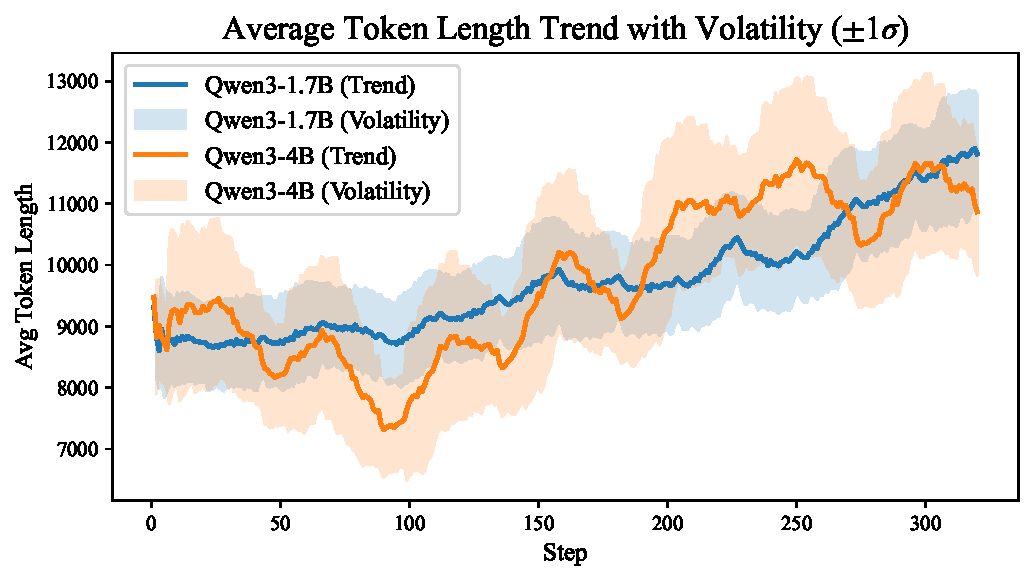
\includegraphics[width=0.9\linewidth]{figures/token_len_trend.pdf}
    \caption{Average response token length trend during training. The solid lines represent the moving average, and the shaded regions indicate the volatility ($\pm 1\sigma$). Both models show a tendency to increase reasoning length as training progresses.}
    \label{fig:token_trend}
\end{figure*}
We implement our training pipeline using the \texttt{verl} (HybridFlow) framework and vllm engine~\citep{sheng2025hybridflow, kwon2023efficient}, which supports efficient reinforcement learning. The specific hyperparameters used for Group Relative Policy Optimization (GRPO) are detailed in Table~\ref{tab:hyperparameters}. We set the group size $G$ (denoted as \texttt{rollout.n} in \texttt{verl}) to 12. Notably, we explicitly set \texttt{use\_kl\_loss=False}, meaning the KL divergence penalty term was disabled during optimization, relying instead on the probability ratio clipping to maintain policy stability. 

We differentiate the batch size for Qwen3-1.7B and Qwen3-4B to accommodate their respective memory footprints. Specifically, the 1.7B model utilizes a larger batch size ($32 \times 12$) compared to the 4B model ($14 \times 12$). This adjustment balances the computational overhead, resulting in comparable training speeds for both architectures; typically, completing 120 training steps requires approximately one day on our 8 $\times$ NVIDIA A100 GPU cluster. Constrained by GPU resources, we conducted a single training run for the main experiments and report results using mean@8 for AIME and mean@4 for the remaining benchmarks.  Throughout the training process, we observed a stable increase in both Solvable Accuracy and Unsolvable Detection Rate.

To further analyze the training dynamics, Figure~\ref{fig:token_trend} illustrates the evolution of the average response token length throughout the training process. We observe a general upward trend for both models, indicating that the RL alignment encourages the generation of more comprehensive reasoning chains (longer CoT) to distinguish solvability. The Qwen3-4B model exhibits higher volatility (indicated by the wider shaded area) compared to the 1.7B model, suggesting more aggressive exploration within the solution space.

To explicitly guide the model's decision-making, we append specific instructions to the system prompt. 
For \textbf{unsolvable detection}, the instruction is: ``\textit{If you believe the problem is unsolvable, please output \texttt{\textbackslash boxed\{unsolvable\}} at the end.}'' 
For \textbf{capability calibration} (refusal), the instruction is: ``\textit{If your chain of thought is still confused after prolonged reasoning and you are likely to get the answer wrong, please provide the final output \texttt{\textbackslash boxed\{Beyond my capabilities\}}.}''. We rely on these predefined output formats to programmatically extract and classify the model's final response.

We will release our dataset, data construction pipeline, and training code upon acceptance.

% ---------------------------
